
\documentclass{beamer}
\usepackage{HECbeamer}
\usepackage{icomma}
\usepackage{numprint}
\title[\color{white}{MATH 60604 \S~6e - Pente aléatoire}]{\texorpdfstring{MATH 60604 \\Modélisation statistique \\ \S~6e - Pente aléatoire}{MATH 60604 \\Modélisation statistique \\ \S~6e - Pente aléatoire}}
\author{Léo Belzile}
\institute{HEC Montréal\\
Département de sciences de la décision}
\date{}


\begin{document}
\frame{\titlepage}
\begin{frame}
\frametitle{Formulation du modèle}
 On considère un modèle linéaire mixte avec ordonnée à l'origine et pente aléatoire pour les données \code{vengeance},
  \begin{align*}
  \bs{Y}_i \mid \bs{\mathcal{B}}_i =\bs{b}_i &\sim \mathsf{No}_{5}\left( \mathbf{X}_i \bs{\beta} + \mathbf{Z}_i\bs{b}_i, \sigma^2 \mathbf{I}_5\right) \\
  \bs{\mathcal{B}}_i & \sim \mathsf{No}_{2}( \bs{0}_2, \bs{\Omega})
 \end{align*}
où $\mathbf{Z}_i = [\bs{1}_5, \code{t}_i]$ est une matrice $5 \times 2$ pour les effets aléatoires et  $\bs{\Omega} = \big( \begin{smallmatrix}\omega_{11} & \omega_{12} \\ \omega_{12} & \omega_{22}\end{smallmatrix}\big)$.

Les colonnes de $\mathbf{Z}_i$ incluent d'ordinaire les variables suivantes:
\bi \item temps
\item indicateurs de variables binaires/catégorielles (effet de groupe).
\ei
\end{frame}
\begin{frame}
\frametitle{Effet aléatoire sur une variable explicative}
Soit la matrice $\mathbf{Z}_i = [\bs{1}_{n_i}, \mathbf{X}_{1i}]$. 
\begin{align*}
Y_{ij}=(\beta_0 +\alert{b_{0i}}) + (\beta_1+\alert{b_{1i}})\mathrm{X}_{ij1}+\beta_2\mathrm{X}_{ij2}+\cdots+\beta_p\mathrm{X}_{ijp} + \varepsilon_{ij}.
\end{align*}
\bi
\item L'effet conditionel de la variable $\mathrm{X}_1$ \alert{pour le groupe $i$} est $\beta_1 + b_{1i}$
\item Le paramètre $\beta_1$ est la « pente » $\mathrm{X}_1$ moyenne pour la population.
\item $\beta_1+b_{1i}$ est l'effet de $\mathrm{X}_1$ spécifique au groupe $i$.
\ei
\end{frame}
\begin{frame}
\frametitle{Covariance de la réponse}
\bi
\item La matrice de covariance de $\bs{Y}_{i}$ dépend des variables explicatives de $\mathbf{Z}_i$ qui induisent un effet aléatoire.
\item Par exemple, si $\mathbf{Z}_{i} = [\bs{1}_{n_i}, \mathbf{X}_{1i}]$, la variance marginale de $Y_{ij}$ est
\begin{align*}
\Va{Y_{ij}\mid \mathbf{X}_i}=\omega_{11}+\mathrm{X}_{ij1}^2 \omega_{22} + 2\mathrm{X}_{ij1} \omega_{12}+\sigma^2_{\varepsilon}.
\end{align*}
\item Si les aléas sont indépendants, la covariance entre deux observations d'un même groupe est 
\begin{align*}
\Co{Y_{ij}, Y_{ik}\mid \mathbf{X}_i}=\omega_{11}+\mathrm{X}_{ij1}\mathrm{X}_{1ik}\omega_{22}+(\mathrm{X}_{ij1}+\mathrm{X}_{1ik})\omega_{12}.
\end{align*}
\item Il peut être difficile d'estimer les paramètres si la structure de covariance de $\bs{Y}_i$ est complexe (en plus des coûts computationnels).
\ei
\end{frame}

\begin{frame}[fragile]
\begin{tcolorbox}[colback=white, colframe=hecblue, title=Code \SASlang{} pour ajuste un modèle avec pente aléatoire]
\begin{verbatim}
proc mixed data=modstat.vengeance;
model vengeance = sexe age vc wom t 
    / ddfm=kenwardroger solution;
random intercept t / subject=id type=un v=1 vcorr=1;
run;
\end{verbatim}
\end{tcolorbox}
La sortie inclut des information sur le nombre de paramètres de covariance, le nombre d'effets aléatoires, etc.
\begin{center}
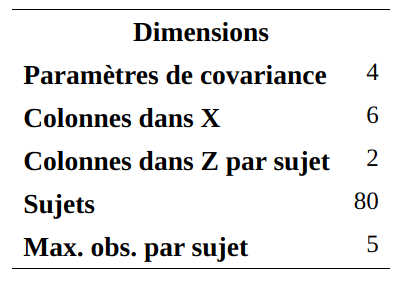
\includegraphics[width = 0.35\linewidth]{img/c6/diapos7-e23}
\end{center}
\end{frame}
% \begin{frame}
%  
% \end{frame}


\begin{frame}
 \frametitle{Matrice de covariance de la réponse}
 \begin{center}
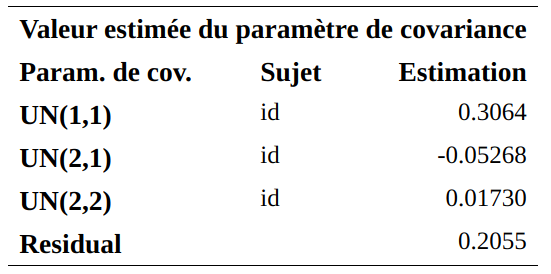
\includegraphics[width = 0.47\linewidth]{img/c6/diapos7-e25}
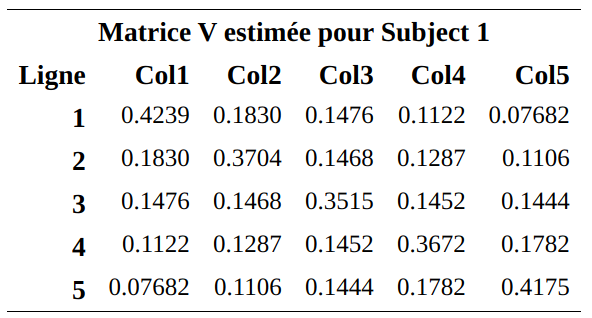
\includegraphics[width = 0.5\linewidth]{img/c6/diapos7-e24}
\end{center}
\bi \item 
La variance de l'effet aléatoire sur l'ordonnée à l'origine est $\omega_{11}=\numprint{0.306}$
\item La variance de l'effet aléatoire sur la pente est $\omega_{22}=\numprint{0.017}$
\item La corrélation entre les deux effets aléatoires est $-\numprint{0.72}$.
\ei
\end{frame}
\begin{frame}
\frametitle{Tester la corrélation entre effets aléatoires}
\bi
\item On peut tester si  $\Hy_0: \omega_{12}=0$ versus $\Hy_a: \omega_{12} \neq 0$ en ajustant un modèle avec matrice de covariance de $\bs{b}_i$ diagonale et en faisant un test de rapport de vraisemblance (REML, car les effets fixes sont les même) \bi 
\item dans \SASlang{}, le modèle de covariance \code{type=vc} (option par défaut pour effets aléatoires).
\item la statistique de test est $R=\numprint{8.98}$ 
\item sa loi nulle asymptotique est $\chi^2_1$ (problème régulier, la covariance peut être négative)
\item la valeur-$p$ est $\numprint{0.002}$:
\item la corrélation entre effets aléatoires est fortement significative. \ei
\ei
\end{frame}
\begin{frame}
\frametitle{Comparaison de modèles}
\bi \item 
 On pourrait comparer avec le modèle qui inclut uniquement un effet aléatoire pour l'ordonnée à l'origine aléatoire
 \bi \item ce qui revient à tester $\Hy_0: \omega_{22} = \omega_{12}=0$.  
 \item La loi nulle asymptotique est  $\frac{1}{2} \chi^2_1 + \frac{1}{2} \chi^2_2$, 
 \item mais l'approximation est mauvaise en échantillon fini\ldots mieux vaut utiliser un critère d'information.
 \ei
 \ei
\end{frame}


\end{document}
